\documentclass[9pt, compress, xcolor=table]{beamer}


\usetheme{m}

\usepackage{amsmath,amssymb,amsthm}
\usepackage{latexsym}
\usepackage{booktabs}
\usepackage[scale=2]{ccicons}
\usepackage{minted}
% \usepackage[utf8]{inputenc}
% \usepackage[T2A]{fontenc}
% \usepackage[english, russian]{babel}
%%% For accessing system, OTF and TTF fonts
%%% (would have been loaded by polylossia anyway)
\usepackage{fontspec}
%%% For language switching -- like babel, but for xelatex
\usepackage{polyglossia}
 %\setmainfont{PT Sans} вообще шрифты определяются в теме бимера
\setmainlanguage{russian}
\setotherlanguages{english} %% or other languages

\usepackage{graphicx}
\usepackage{xcolor}
\usepackage{euscript}
% \DeclareMathOperator{\arctg}{arctg}
\usepackage{tabu} % https://ru.sharelatex.com/learn/Tables
\DeclareGraphicsExtensions{.pdf,.jpg,.png}
\graphicspath{{../images/}{./images/}}

\colorlet{Mycolor1}{green!50!blue!50!}
\DeclareMathOperator{\Ima}{Im}
\usemintedstyle{trac}

\title{Физические принципы микроскопии сверхвысокого разрешения}
\subtitle{осенний семестр, 2018}
\author{ассистент, к.ф.-м.н. Шутова О.А.}
\institute{МГУ им. М.В. Ломоносова, физический факультет}

\begin{document}

\maketitle

\plain{}{Лекция 7. Электродинамика плазмонных материалов с точки зрения микроскопии сверхразрешения}

\begin{frame}{Веселаго, 1967}

Веселаго в 1967 году высказал предположение, что одновременная смена знаков $\epsilon$ и $\mu$ не противоречит законам природы (и, значит, существование таких веществ
возможно) и существенно влияет на его физические свойства.
\begin{center}
\begin{equation*}
n^2 = \epsilon \mu \quad \vec k \times \vec H = \omega \epsilon \vec E\quad \vec k \times \vec E = -\omega \mu \vec H \quad \vec S = \frac{c}{4 \pi}\left[\vec E \vec H\right]
\end{equation*}
\begin{equation*}G = \begin{pmatrix} \alpha_1 & \alpha_2 & \alpha_3\\
\beta_1 & \beta_2 & \beta_3\\ \gamma_1 & \gamma_2 & \gamma_3
\end{pmatrix} \qquad p = det G\quad p=1\Rightarrow RHM \quad p= -1\Rightarrow LHM
\end{equation*}
\begin{equation*}
\frac{\sin \varphi}{\sin \psi} = \frac{n_2}{n_1}
\quad \Rightarrow \quad\frac{\sin \varphi}{\sin \psi} = \frac{p_1}{p_2}\frac{n_2}{n_1}
\end{equation*}
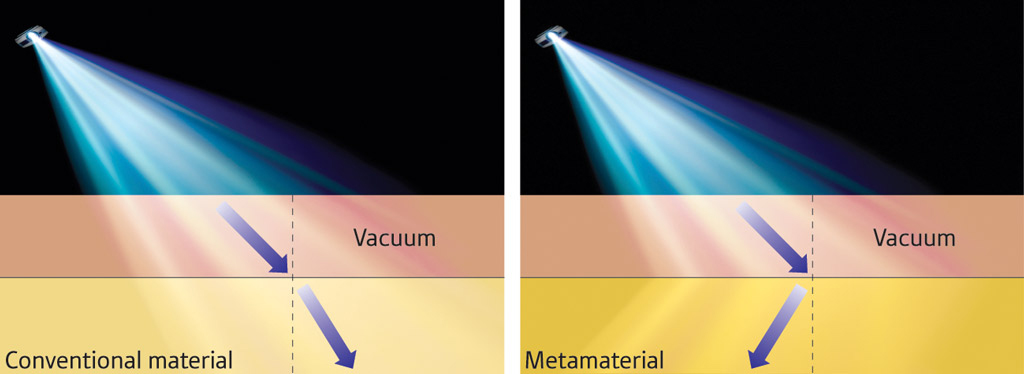
\includegraphics[width=0.6\textwidth]{neg_ref_1}
\end{center}

\end{frame}


\begin{frame}{Источники}
    
    Фундаментальные обзоры по электродинамике метаматериалов:
    \begin{itemize}
        \item В.Г. Веселаго. Электродинамика веществ с одновременно отрицательными $\epsilon$ и $\mu$. \textit{Успехи физических наук.} 1967.
        \item В.Г. Веселаго. Волны в метаматериалах: роль в современной физике. \textit{Успехи физических наук.} 2011.
        \item В.М. Агранович, Ю.Н. Гарштейн. Пространственная дисперсия и отрицательное преломление света. \textit{Успехи физических наук.} 2006.
        \item А.Н. Лагарьков и др. Электрофизика и электродинамика метаматериалов. ИТПЭ РАН. 2010.
        \item М.А. Ремнёв, В.В. Климов. Метаповерхности: новый взгляд на уравнения Максвелла и новые методы управления светом. \textit{Успехи физических наук.} 2018.
    \end{itemize}
    
    
\end{frame}

\begin{frame}{Особенности преломления и эффекта Доплера}


\begin{columns}[c]
\column{6cm}
\begin{center}
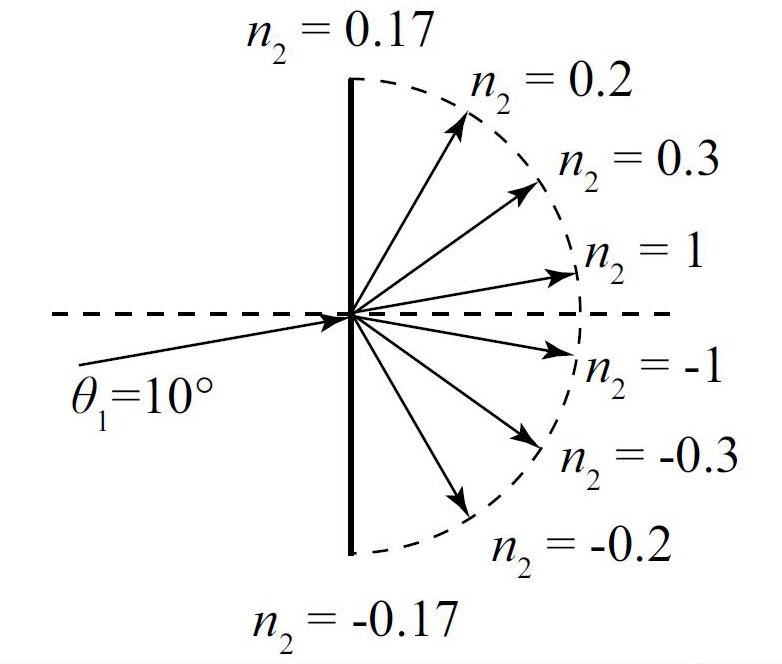
\includegraphics[width=0.5\textwidth]{neg_ref_2}
\end{center}
Такие свойства означают, главным образом, что фазовая скорость в таких материалах противонаправлена переносу энергии. Волна, фазовая скорость которой направлена противоположно направлению переноса энергии, называется \textcolor{red!50!black}{обратной волной (backward wave)}. Впервые описана более 100 лет назад Лэмбом.
\column{6cm}
\begin{center}
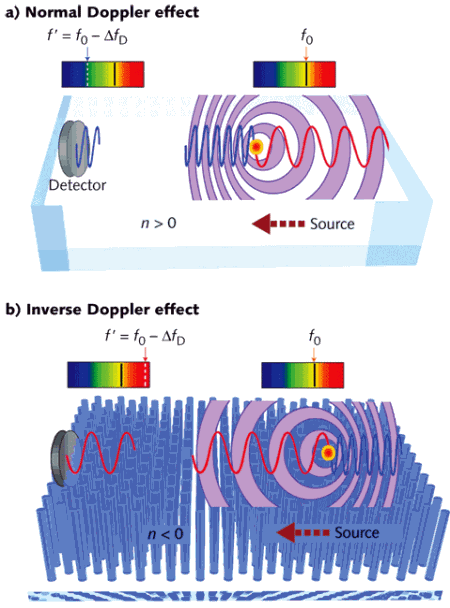
\includegraphics[width=5cm]{neg_ref_6}
\end{center}
\end{columns}
Если паровоз резко замедлится, то дым из его трубы придет раньше, чем он сам. Это, конечно, лишь аналогия. Впрочем, плазмонные материалы - это и есть вещества, замедляющие свет.

\end{frame}

\begin{frame}{Плоскопараллельный слой метаматериала}

\begin{columns}[c]
\column{6cm} Рассмотрим плоскопараллельную пластину: слева и справа от нее пусть $n=1$, а внутри
$n=-1$, в этом случае углы равны:
\begin{center}
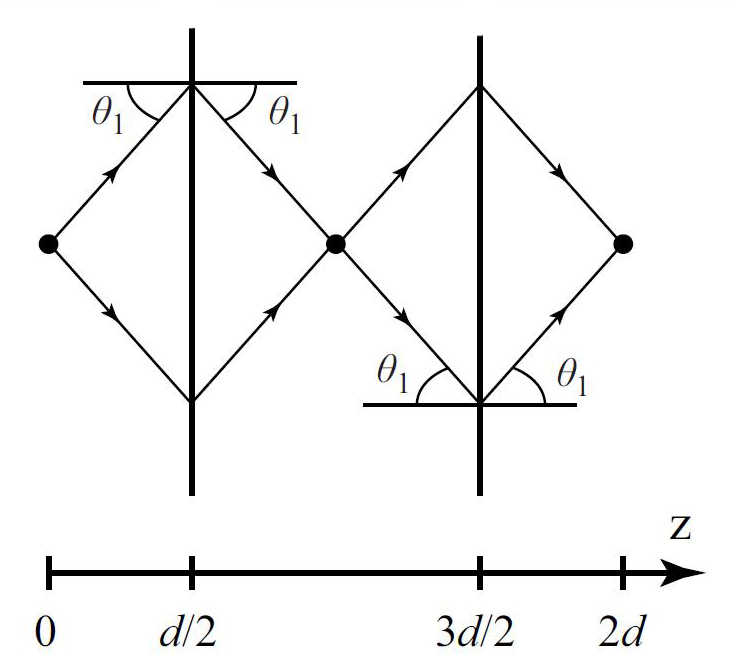
\includegraphics[width=4cm]{neg_ref_3}
\end{center}

Слева и справа от пластины с "<левым"> веществом находятся \textcolor{red}{источники}, а в центре -
\textcolor{blue}{сток}



\column{6cm}

\begin{center}
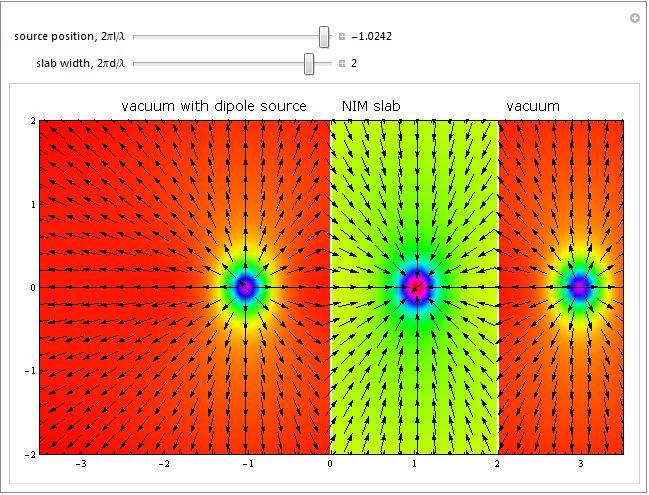
\includegraphics[width=3.8cm]{neg_ref_4}
\end{center}
\begin{center}
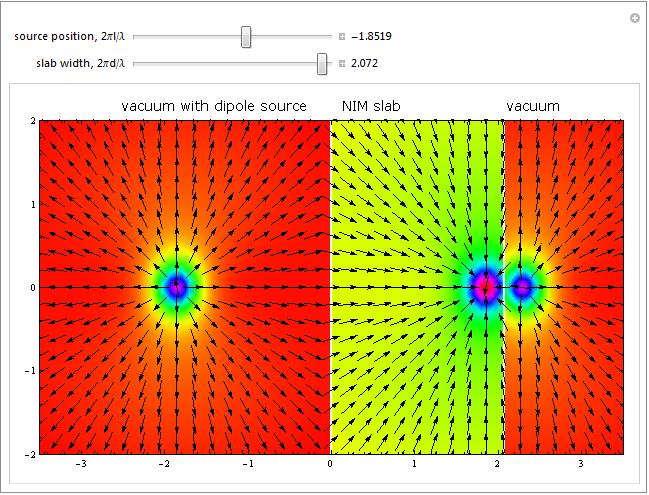
\includegraphics[width=3.8cm]{neg_ref_5}
\end{center}
Wolfram Demonstrations
\end{columns}

\end{frame}

\begin{frame}{Оптическое маскирование}
    \begin{center}
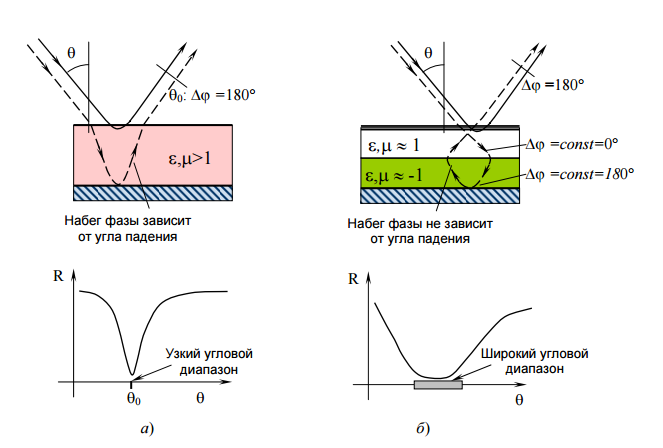
\includegraphics[width=\textwidth
]{mask}
\end{center}
Слева классическое оптическое просветление за счет интерференции, справа - оптическое маскирование на метаматериале.

\end{frame}

\begin{frame}{Sir John Pendry, 2000}

Negative Refraction Makes Perfect Lense, Physical Review Letters, 2000.

\begin{columns}[c]
\column{6cm}
\begin{center}
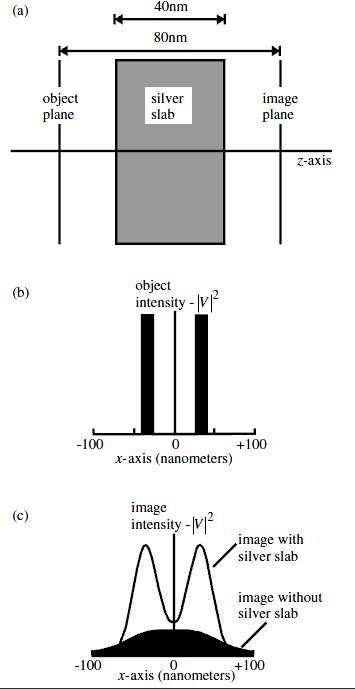
\includegraphics[width=0.5\textwidth]{neg_ref_13}
\end{center}
 $\epsilon \approx 5.7 - 9^2 \omega^{-2} +0.4 \imath$

картина восстановления на частоте $\omega_{rec} = 3.48$ эВ
\column{6cm}



\textcolor{red!50!black}{Основная идея}: в такой среде будут усиливаться эванесцентные волны.

Идеальная линза - это теоретическая модель оптического прибора, который осуществляет такую передачу
изображения объекта, что пространственный спектр объекта и его изображения совпадают. При этом
пропагатор (функция передачи) является константой.

\end{columns}
\end{frame}
\begin{frame}{Идеальная линза Пендри}

\begin{columns}[c]
\column{6cm}

Рассмотрим ситуацию, когда $\epsilon_r = -1$, и $\mu_r = -1$ в слое вещества
\begin{center}
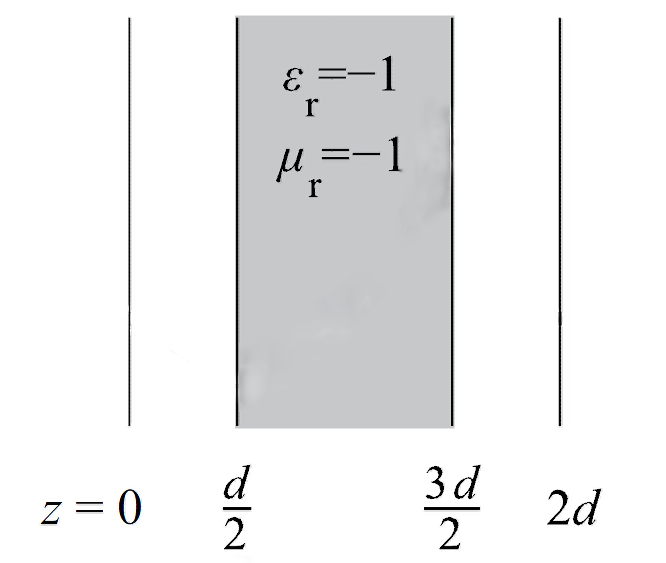
\includegraphics[width=4cm]{neg_ref_40a}
\end{center}

\column{6cm} граничные условия: $k_x = k_{x1}= k_{x2} = K_{x3}$

\textcolor{blue}{среда 1} ($\epsilon_1 = \epsilon_0$, $\mu_1 = \mu_0$): $k_{z1} =
\sqrt{\frac{\omega^2}{c^2}-k_{x}^2}$

\textcolor{blue}{среда 2} ($\epsilon_1 = -\epsilon_0$, $\mu_1 = -\mu_0$): $k_{z1} =
\sqrt{\frac{\omega^2}{c^2}-k_{x}^2}$

\textcolor{blue}{среда 3}($\epsilon_1 = \epsilon_0$, $\mu_1 = \mu_0$): $k_{z3} = k_{z1}$
\begin{center}
$H=H_1H_2H_3$

$H_1= \exp^{-\frac{\imath k_z d}{2}};\quad H_2= \exp^{\imath k_z d};\quad H_3= \exp^{-\frac{\imath
k_z d}{2}}$

$H=1$
\end{center}

\end{columns}
\end{frame}

\begin{frame}{Что в случае эванесцентных волн?}

\begin{columns}[c]

\column{6cm}

\begin{center}
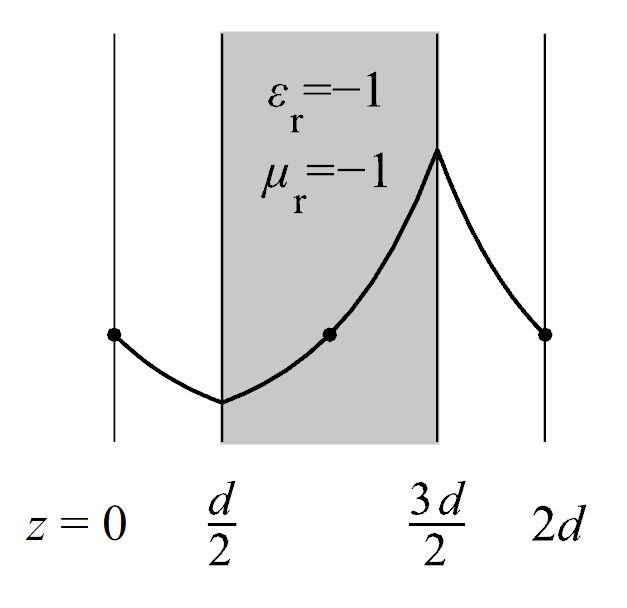
\includegraphics[width=4cm]{neg_ref_40}
\end{center}

\column{6cm}  $k_x>k_0$, волновые вектора вдоль $z$ становятся мнимыми, так что

$k_{z1}\rightarrow \imath k_1$, а $k_{z2}\rightarrow \imath k_2$ тогда

\begin{center}
$H=H_1H_2H_3$

$H_1= \exp^{-\frac{\imath k_z d}{2}};\quad H_2= \exp^{\imath k_z d};\quad H_3= \exp^{-\frac{\imath
k_z d}{2}}$

$H=1$
\end{center}
\textcolor{red}{Функция передачи по прежнему 1!} 
\end{columns}

\begin{center}
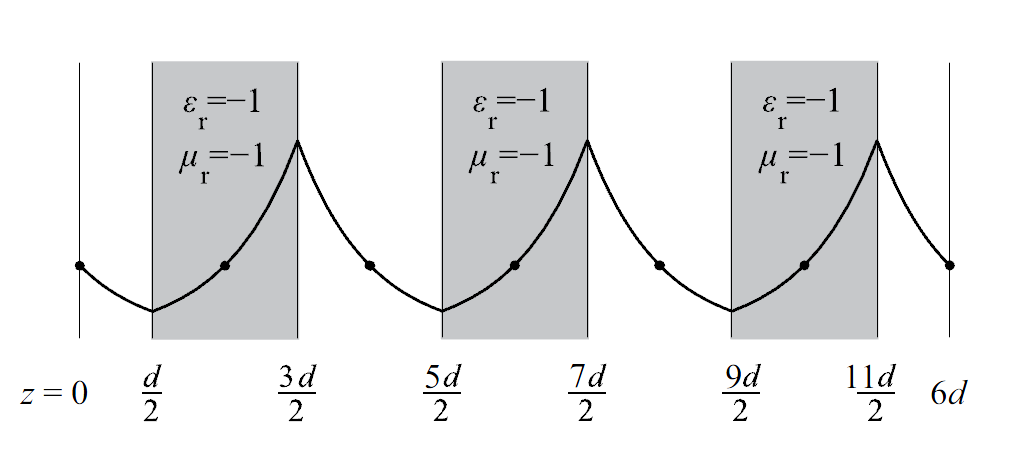
\includegraphics[width=7cm]{neg_ref_40b}
\end{center}

\end{frame}

\begin{frame}{Интенсивность поля внутри линзы Веселаго и линзы Пендри}

\begin{columns}[c]

\column{8cm}
\begin{center}
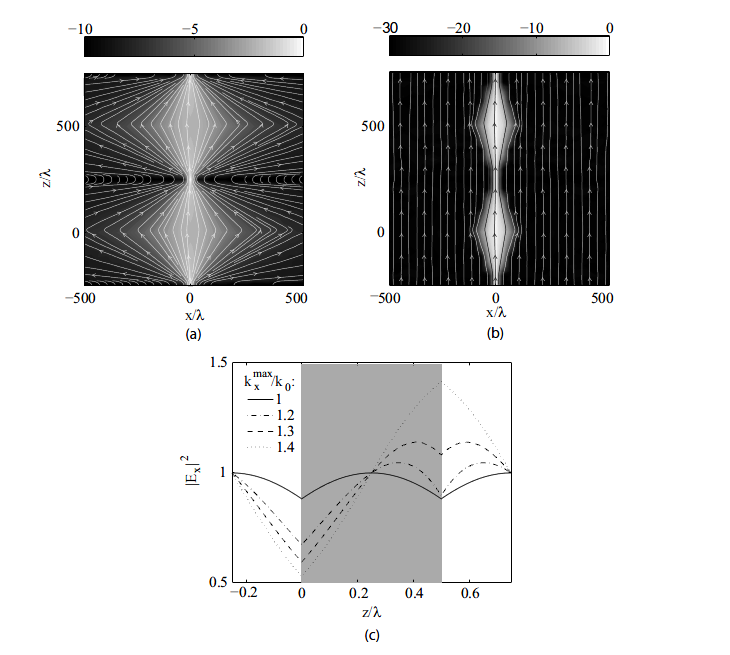
\includegraphics[width=8cm]{neg_ref_40d}
\end{center}

\column{4cm}  (a) и (b) вектор Пойтинга для плоской линзы размером $d/\lambda = 500$, слева
объект размером одна длина волны, справа - пять длин волн (дальнее поле, линза Веселаго), (c)
Модуль поля в зависимость от расстояния вдоль направления распространения при $d/\lambda = 0.5$,
объект размером десятая длины волны (ближнее поле, линза Пендри)
\end{columns}
\end{frame}


\begin{frame}{Учет потерь от идеальной линзы к супер- и гиперлинзам}
\begin{center}
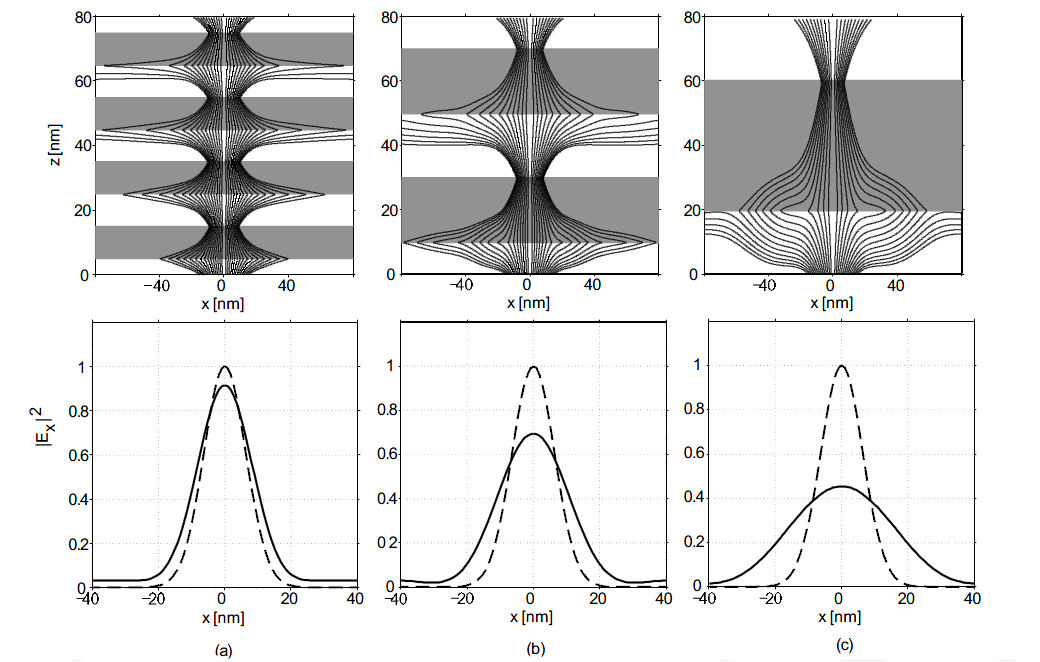
\includegraphics[width=7cm]{neg_ref_40f}
\end{center}

 Суперлинза общей толщиной $80$ нм. (а) Четыре слоя серебра толщиной по 10 нм,
разделенные 10 нм воздуха, (b) два слоя серебра по 20 нм, разделенные 20 нм воздуха, (c) 40 нм
серебра и по 20 нм воздуха с каждой стороны. $\epsilon_r = -1-\imath 0.1$
\end{frame}

\plain{}{Физика вещества с отрицательным показателем преломления}

\begin{frame}{Как получить отрицательные воcприимчивости?}
\begin{center}
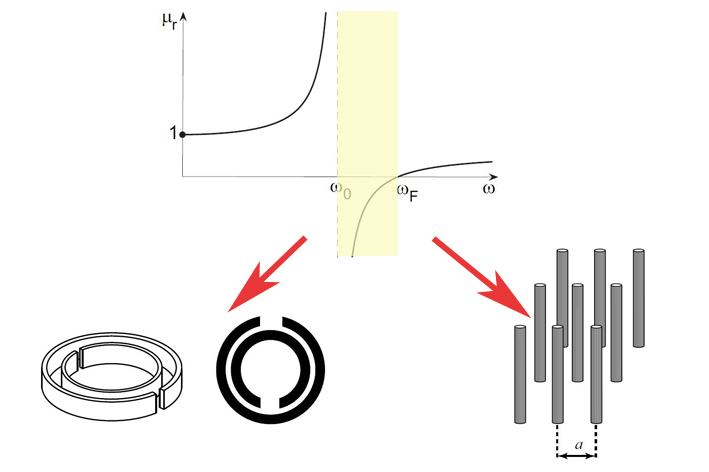
\includegraphics[width=7.5cm]{neg_ref_7d}
\end{center}

\begin{columns}[c]
\column{5.5cm} \begin{block}{\textcolor{red}{Pendry, 1999}} SRR - split-ring resonator
$\omega_p^2 = \frac{2}{\pi r_0^2 L C_{pu}}$, $r_0$ - средний радиус, $L$ -индуктивность, $C_{pu}$ -
емкость пространства между кольцами на единицу длины: $\mu < 0$\end{block}

\column{5.5cm}\begin{block}{\textcolor{red}{Rotman, 1962}} обнаружил, что система
металлических стержней ведет себя как плазма с частотой $\omega_p^2 = \frac{1}{\epsilon_0 a L_w}$:
$\epsilon < 0$\end{block}
\end{columns}
\end{frame}

\begin{frame}{}

 \textcolor{red}{Smith, 2000} предложил соединить эти две системы, чтобы получить $\mu
< 0$ и $\epsilon < 0$ \textcolor{red}{одновременно}.
\begin{columns}[c]
\column{6cm}
\begin{center}
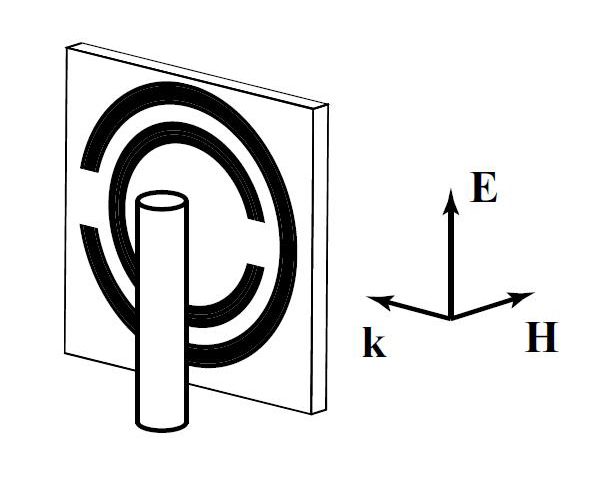
\includegraphics[width=3cm]{neg_ref_7}
\end{center}
Сплошная кривая - только SRR, пунктирная SRR+стержни $\Rightarrow$
\column{6cm}
\begin{center}
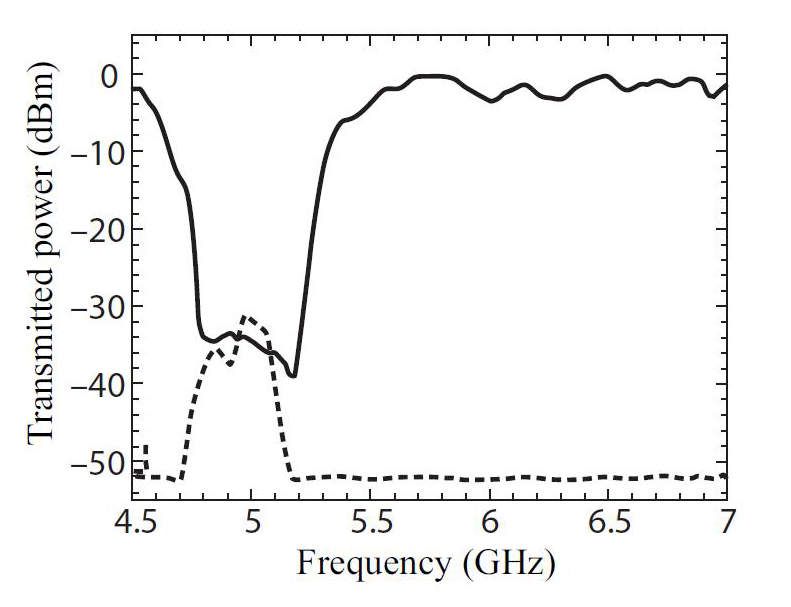
\includegraphics[width=4.5cm]{neg_ref_8}
\end{center}
\end{columns}
\begin{center}
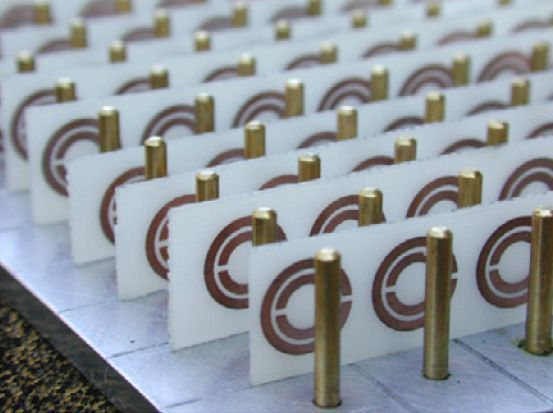
\includegraphics[width=5cm]{neg_ref_21}
\end{center}

\end{frame}

\begin{frame}{}

 \textcolor{red}{Shelby, 2001}: метаматериал в области СВЧ, геометрия призмы
\begin{center}
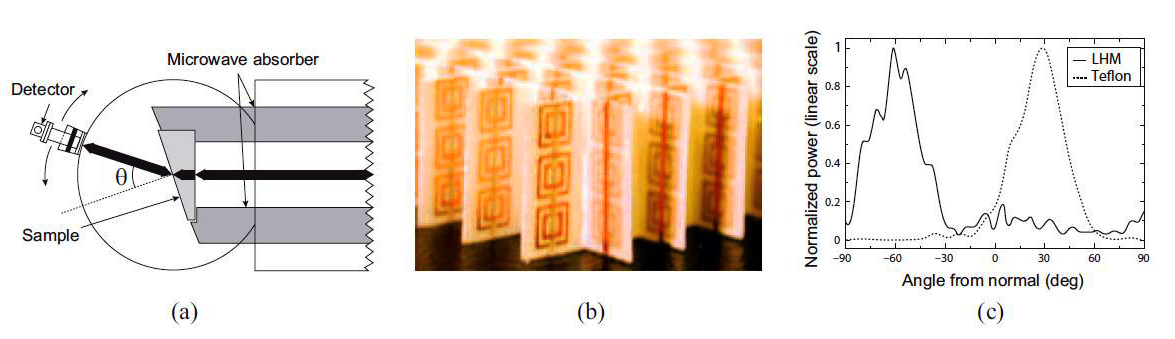
\includegraphics[width=11.5cm]{neg_ref_9}
\end{center}

\begin{center}
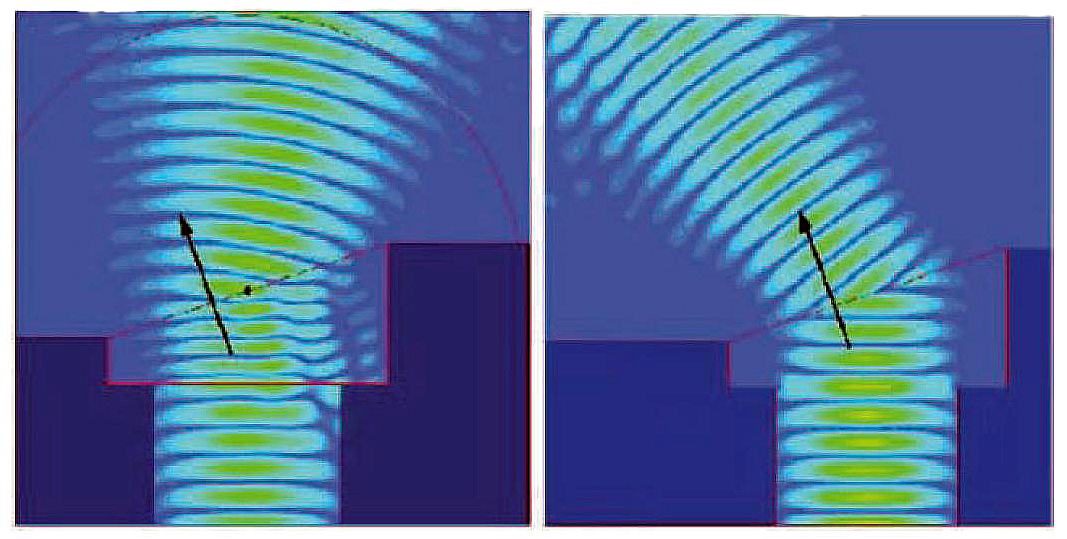
\includegraphics[width=7cm]{neg_ref_10}
\end{center}
\end{frame}

\begin{frame}{}

 \textcolor{red}{Shalaev, 2005; Liu, 2008; и др.}: переход к трехмерным структурам,
выход в оптический диапазон
\begin{columns}[c]
\column{6cm}
\begin{center}
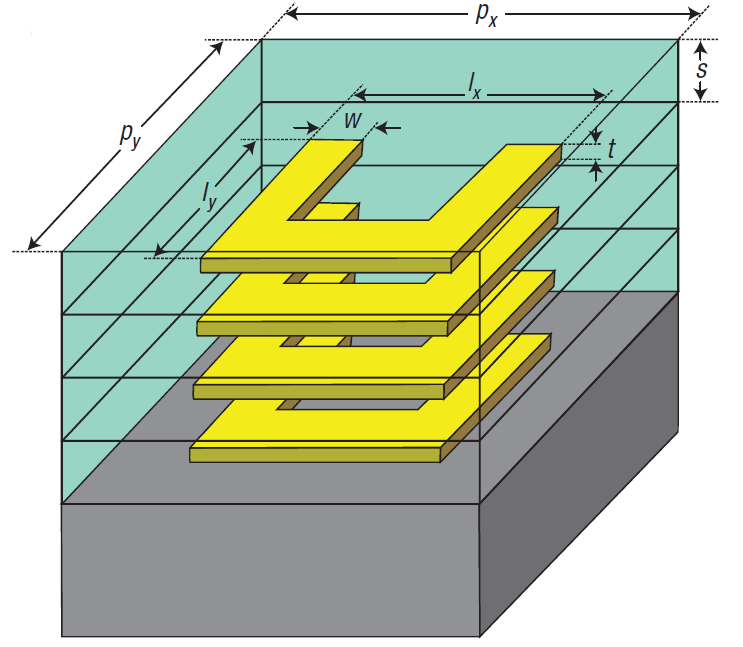
\includegraphics[width=3cm]{neg_ref_34}
\end{center}
Два способа возбуждения мод: поляризация перпендикулярно зазору и параллельно

\column{6cm}
\begin{center}
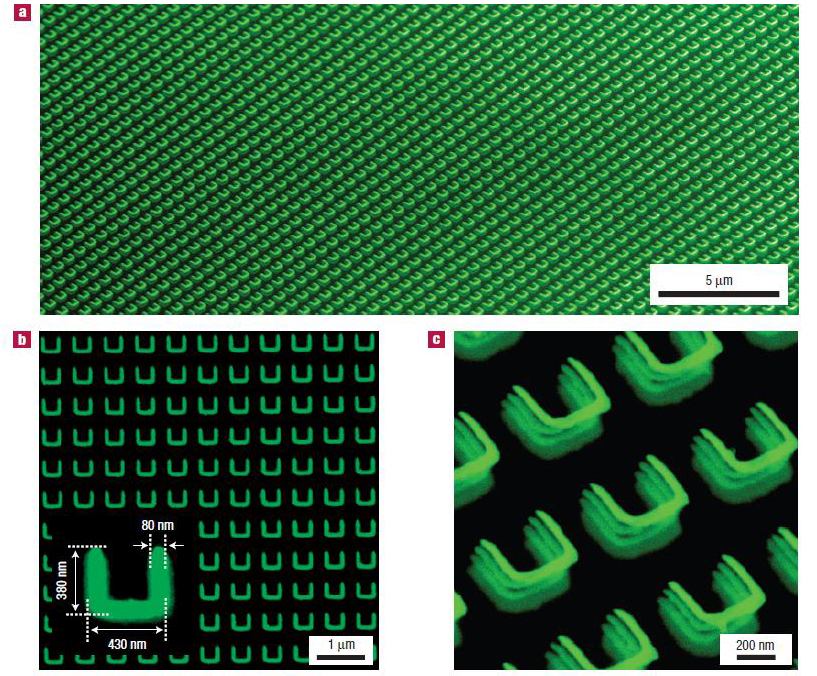
\includegraphics[width=4cm]{neg_ref_36}
\end{center}
\end{columns}
\begin{center}
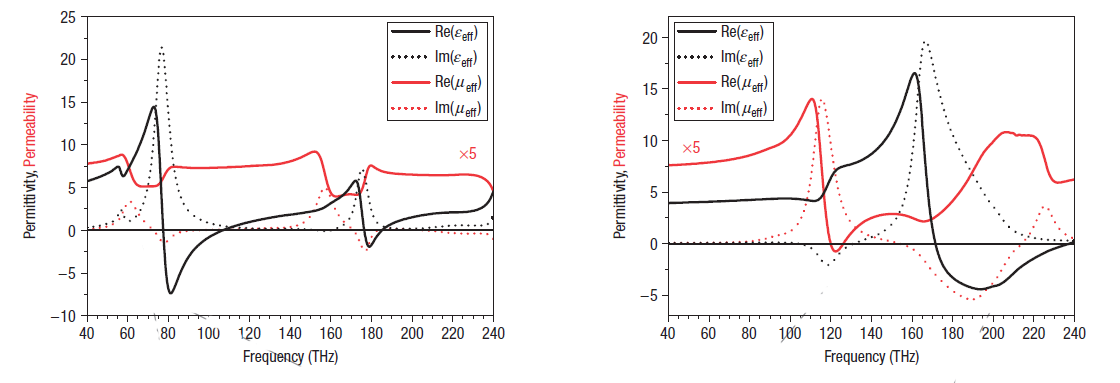
\includegraphics[width=9.5cm]{neg_ref_37}
\end{center}

\end{frame}

\begin{frame}{Метаматериал типа fishnet}

{\scriptsize Университет Беркли, 2008, J. Valentine и др.}

\begin{columns}[c]
\column{6cm}
\begin{center}
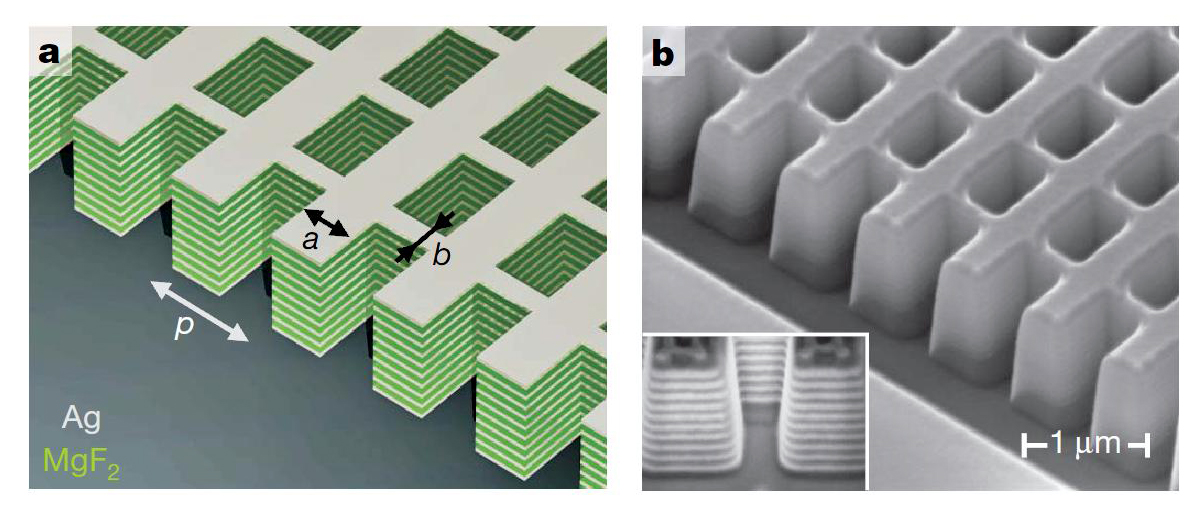
\includegraphics[width=5cm]{neg_ref_24}
\end{center}
 Схема и СТМ изображение структуры типа fishnet. Это 21-слойный материал, размер ячейки
$p=860$ нм, $a=565$ нм, $b = 265$ нм. В слоях чередуется серебро ($Ag$) с фторидом магния
($MgF_2$)

\column{6cm}
\begin{center}
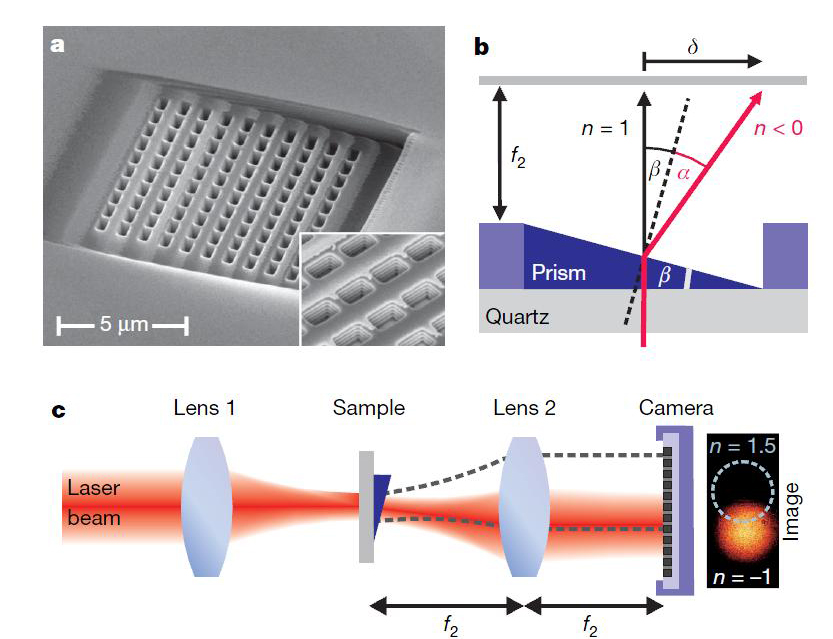
\includegraphics[width=5cm]{neg_ref_25}
\end{center}

 Схема эксперимента по измерению оптических свойств метаматериала типа fishnet
\end{columns}
\end{frame}

\begin{frame}{Метаматериал типа fishnet}

\begin{columns}[c]
\column{6cm}
\begin{center}
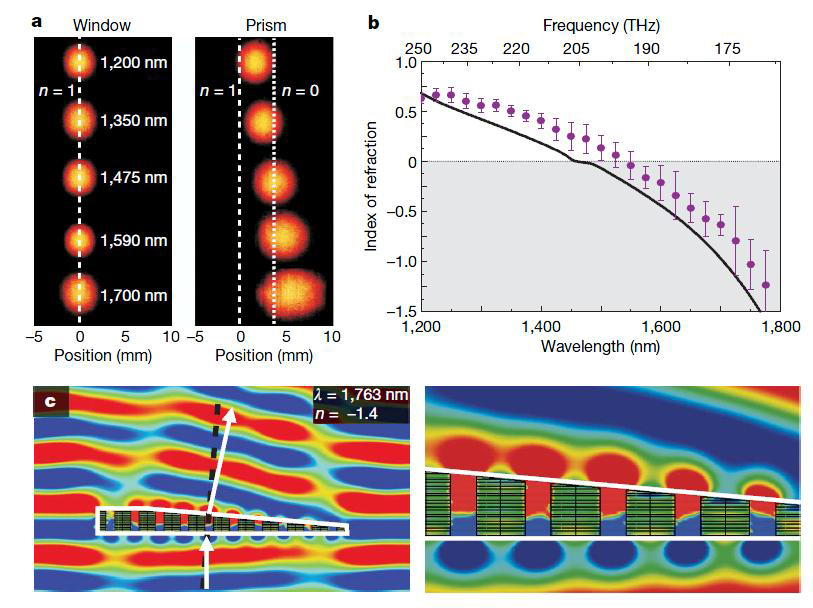
\includegraphics[width=6cm]{neg_ref_26}
\end{center}
Результаты эксперимента и моделирование поля в призме из метаматериала

\column{6cm}
\begin{center}
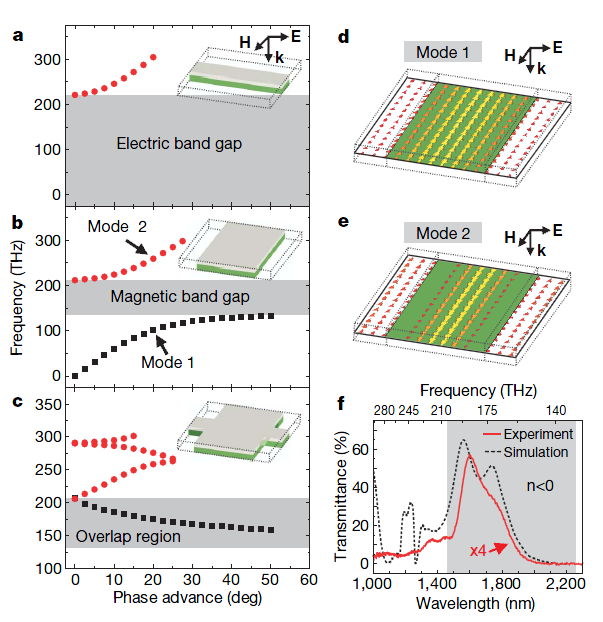
\includegraphics[width=5cm]{neg_ref_26a}
\end{center}

Дисперсионные кривые: (a) для металлических проводов, вытянутых вдоль поля $\vec E$, (b)
полосок, вытянутых вдоль поля $\vec H$, и комбинация. Производная кривой в области перекрытия
запрещенных зон - отрицательная
\end{columns}

\end{frame}


\begin{frame}{Сумма сложностей в оптическом диапазоне}

В оптическом диапазоне мы наталкиваемся на три трудно разрешимые проблемы:

\begin{itemize}
\item проблема, которую мы и раньше уже затрагивали в связи с переходом к оптическим антеннам, это большие потери при распространении ЭМ через вещество в оптическом диапазоне

\item отсутствие естественного магнетизма в оптическом диапазоне, т.е. в оптике мы, как правило, всегда полагаем $\mu=1$

\item частотная избирательность отклика в оптическом диапазоне при желательности распространить указанные закономерности на весь видимый диапазон, т.к. объекты, которые мы собираемся изучать не обязаны быть одноцветными
\end{itemize}

Для получения магнетизма нам необходимо наличие индуктивных элементов. Рассмотрим отклик двух параллельных наностерженьков.  

\end{frame}

\begin{frame}{Реализация обобщенного закона Снеллиуса}
  \begin{center}
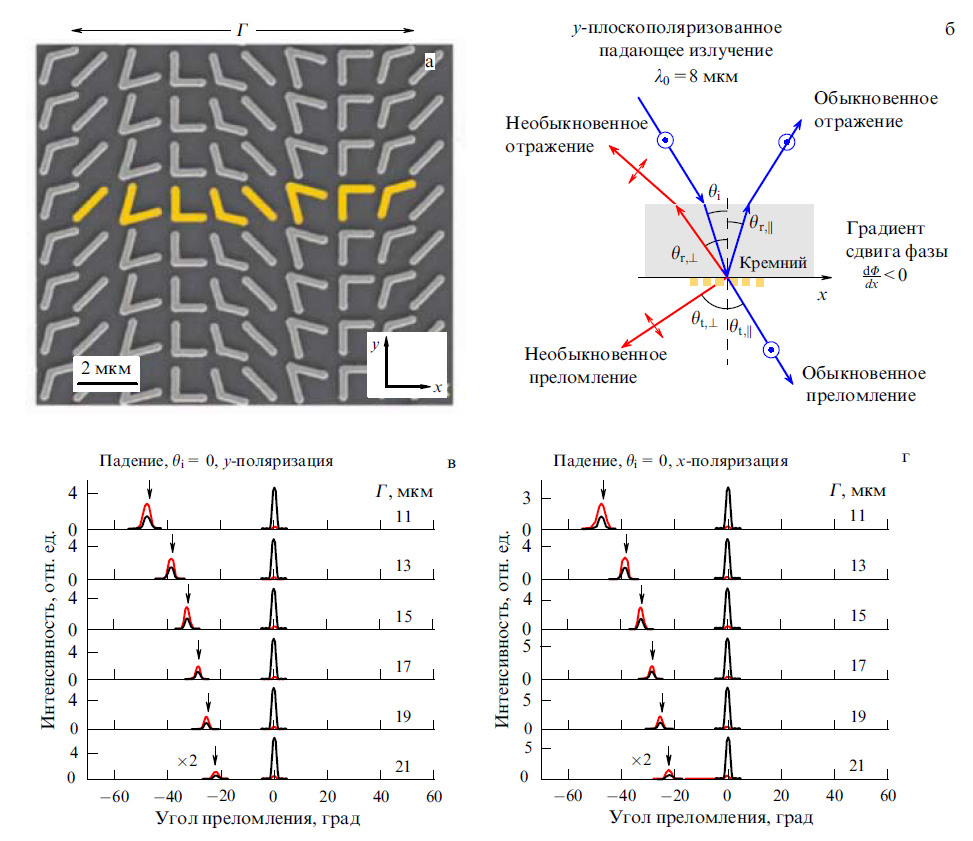
\includegraphics[width=0.9\textwidth]{nanorod2}
\end{center}  
\end{frame}

\begin{frame}{Отклик пары параллельных стерженьков при нормальном падении поля}

\begin{columns}[c]
\column{7cm}
\begin{center}
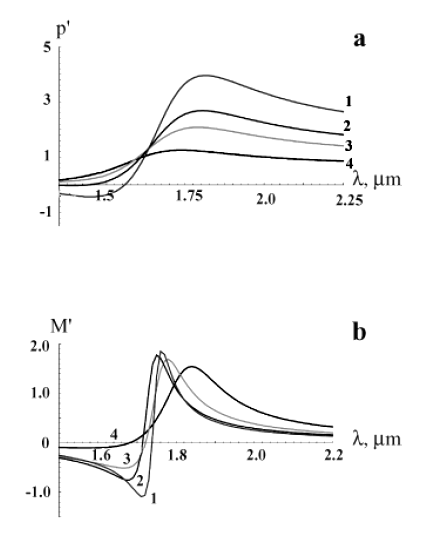
\includegraphics[width=\textwidth]{neg_ref0}
\end{center}
\column{5.5cm}
\begin{center}
Длина стерженьков $a=0.35$ мкм, диаметр $b=0.05$ мкм, 

варьируется расстояние между ними: (1) $d=0.15$ мкм, (2) $d=0.23$ мкм, (2) $d=0.3$ мкм, (4) $d=0.45$ мкм

\begin{equation*}
R=\left|\frac{2 d k (\epsilon-\mu)}{(-2+\imath d k \epsilon)(-2+\imath d k \mu)}\right|^2
\end{equation*}
\begin{equation*}
T=\left|\frac{4+ d^2 k^2 \epsilon\mu}{(-2+\imath d k \epsilon)(-2+\imath d k \mu)}\right|^2
\end{equation*}
\end{center}

А.К. Сарычев, В.М. Шалаев, \textbf{Электродинамика метаматериалов}, 2011 (русский перевод)

\end{columns}
\end{frame}


\section{Анизотропные метаматериалы}

\begin{frame}{Гиперболические среды}

Гиперболические среды - это анизотропные метаматериалы (АММ).

Два класса - диэлектрические АММ (одна из трех компонент тензора восприимчивости отрицательна, I) и металлические АММ (две из трех компонент тензора восприимчивости отрицательны, II)

\begin{center}
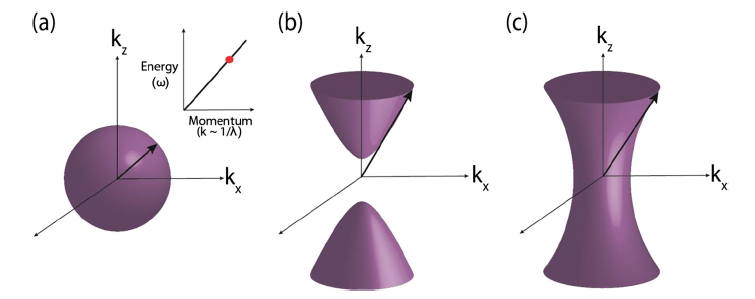
\includegraphics[width=0.7\textwidth]{neg_ref_n5}

 a - обычный диэлектрик
b - АММ I типа: $\epsilon_{zz}<0, \epsilon_{xx},\epsilon_{yy}>0$
b - АММ II типа: $\epsilon_{zz}>0, \epsilon_{xx},\epsilon_{yy}<0$
\end{center}
\begin{equation*}
\frac{k_x^2+k_y^2}{\epsilon_{zz}}+\frac{k_z^2}{\epsilon_{xx}}=\frac{\omega^2}{c}
\end{equation*}

{\scriptsize Z.Jacob et al. Hyperbolic metamaterials: fundamental and appications, 2014

V. Drachev et al. Hyperbolic metamaterials: new physics behind a classical problem, 2013}
\end{frame}

\begin{frame}{Теория эффективной среды}
\begin{columns}
\column{6.5cm}
\begin{center}
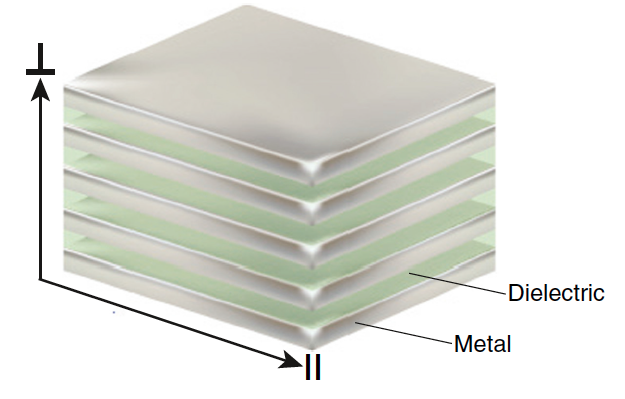
\includegraphics[width=0.6\textwidth]{neg_ref_n9}
\begin{equation*}
\rho=\frac{d_m}{d_m+d_d}
\end{equation*}
\begin{equation*}
\epsilon_{||}=\rho\epsilon_m+(1-\rho\epsilon_d)
\end{equation*}
\begin{equation*}
\epsilon_{\perp}=\frac{\epsilon_m \epsilon_d}{\rho\epsilon_d+(1-\rho)\epsilon_m)}
\end{equation*}
Металл: серебро, толщина серебра 20 нм, толщина диэлектрика (диоксид титана) 40 нм.
\end{center}
\column{6.5cm}
\begin{center}
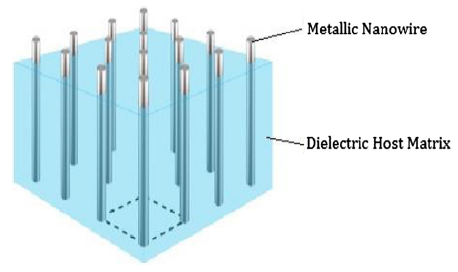
\includegraphics[width=0.6\textwidth]{neg_ref_n10}
\begin{equation*}
\rho=\frac{a}{A}
\end{equation*}
\begin{equation*}
\epsilon_{||}=\frac{(1+\rho)\epsilon_m \epsilon_d+(1-\rho \epsilon_d^2)}{(1+\rho)\epsilon_d+(1-\rho)\epsilon_m)}
\end{equation*}
\begin{equation*}
\epsilon_{\perp}=\rho\epsilon_m+(1-\rho\epsilon_d)
\end{equation*}
Металл: золото, расстояние между стерженьками 40-70 нм, диаметр 10-50 нм, длина 20-700 нм.
\end{center}
\end{columns}
\textcolor{red!50!black}{Порог перколяции} - критическая концентрация металла, внедренного в диэлектрик, при которой начинает проявляться металлическое поведение.
\end{frame}

\begin{frame}{Диэлектрические восприимчивости и кривая отражения}
\begin{center}
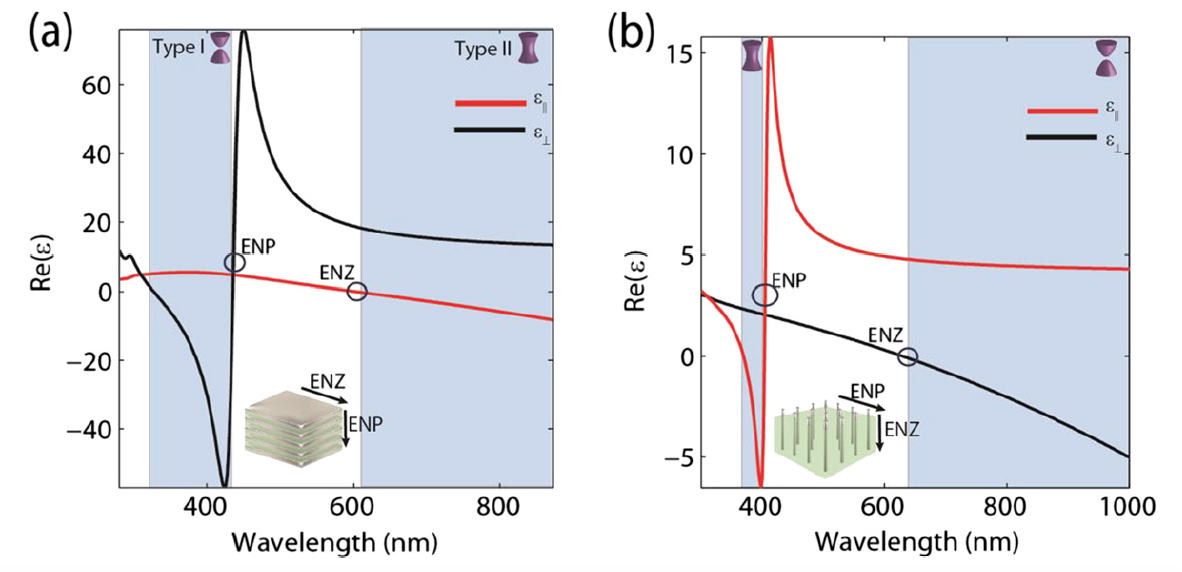
\includegraphics[width=0.7\textwidth]{neg_ref_n2}

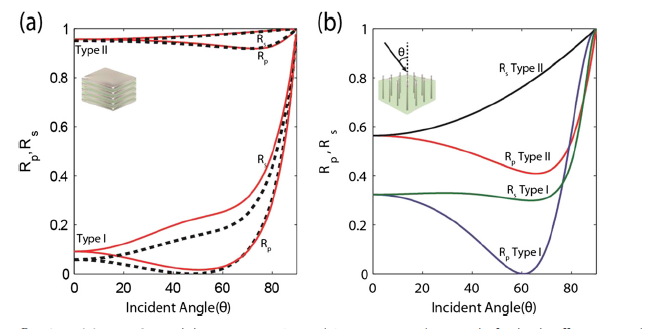
\includegraphics[width=0.7\textwidth]{neg_ref_n7}
\end{center}
\end{frame}

\begin{frame}{Моделирование пропускающей способности слоистой системы}
\begin{center}
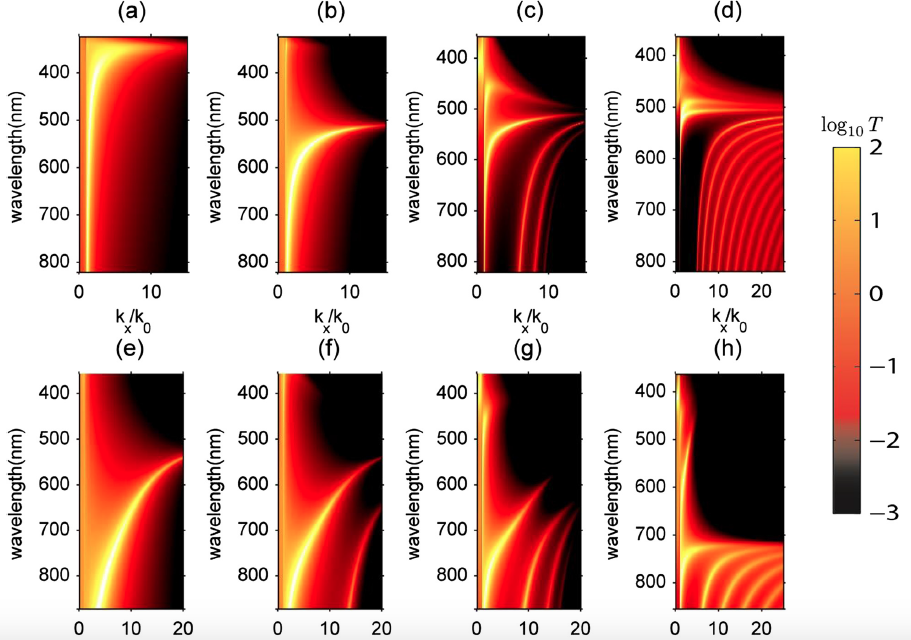
\includegraphics[width=0.7\textwidth]{neg_ref_n3}

(a) 30 нм Ag; (b) 30 нм Ag; 30 нм $TiO_2$; (c) 8 таких слоев; (d) такой же как в (с) толщины по теории эффективной среды с $50\%$ заполнения; 

(e) 10 нм Ag; 30 нм $TiO_2$; (f) 4 слоя; (g) 8 слоев; (h)такой же как в (g) толщины по теории эффективной среды с $25\%$ заполнения;
\end{center}
\end{frame}

\begin{frame}{Визуализация со сверхразрешением}
\begin{center}
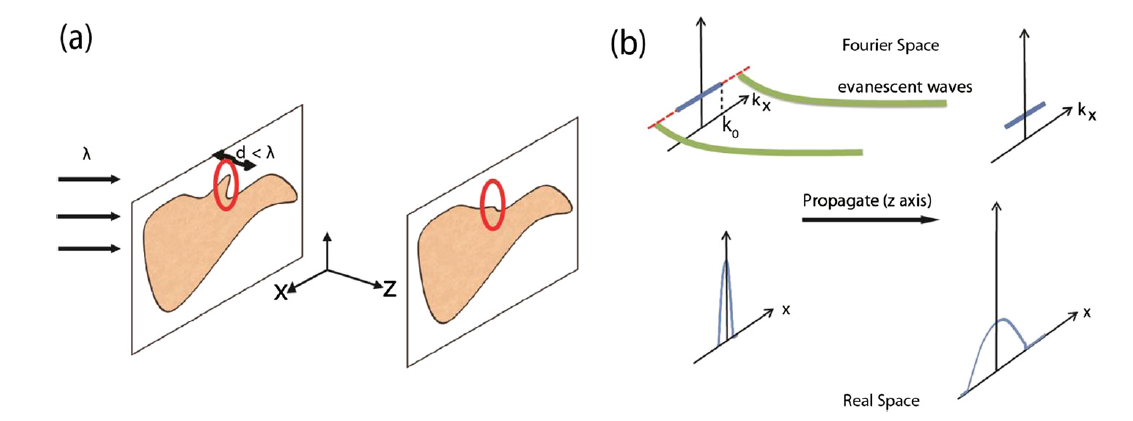
\includegraphics[width=0.7\textwidth]{neg_ref_n4}

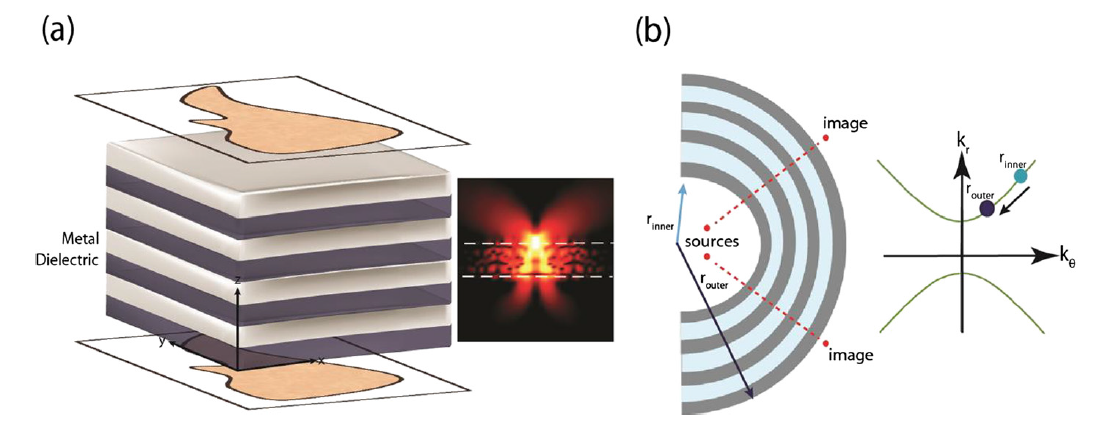
\includegraphics[width=0.7\textwidth]{neg_ref_n1}
\end{center}
\end{frame}


\begin{frame}{Работа группы Jacob}
\begin{center}
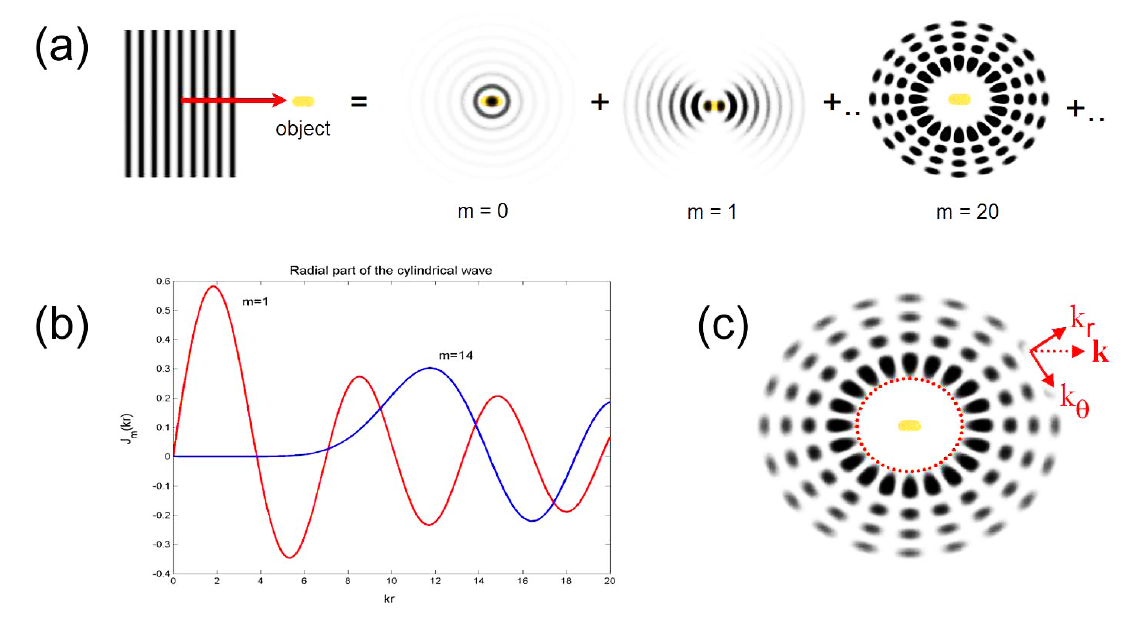
\includegraphics[width=8cm]{neg_ref_43}
\end{center}

\begin{center}
\begin{equation*}
\exp (\imath k x) = \sum_{m=-\inf}^{m=\inf} \imath^m J_m(kr) \exp(\imath m \phi)
\end{equation*}
\end{center}
экспоненциальное затухание высоких $m-$мод связано с законом сохранения: $m=k_{\theta}r$,
$k_{\theta}\propto 1/r$
\end{frame}

\begin{frame}{}
\begin{columns}[c]

\column{6cm}
\begin{center}
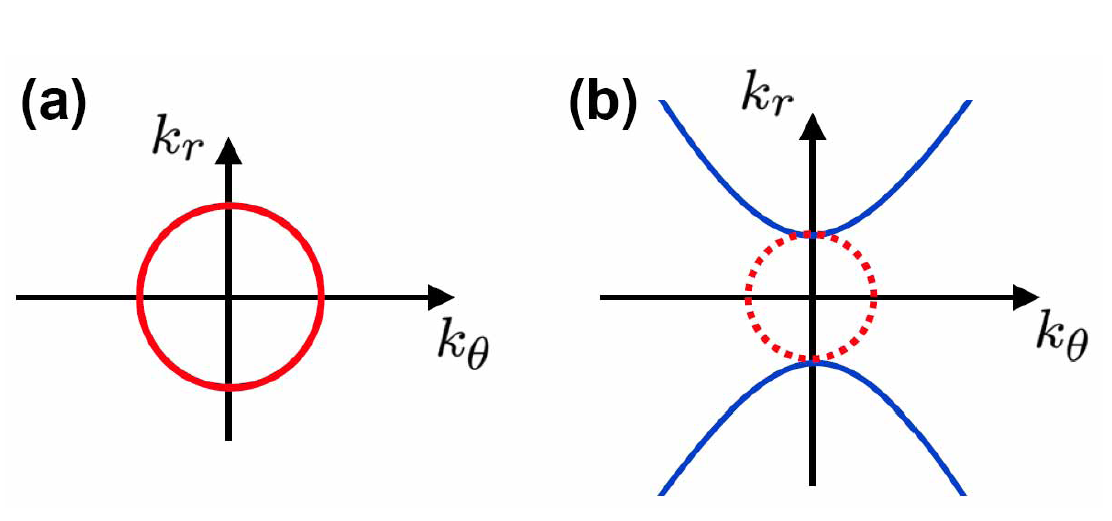
\includegraphics[width=5.5cm]{neg_ref_44}
\end{center}
Дисперсионная кривая для изотропной среды (а) и среды с $\epsilon_r<0$, а
$\epsilon_{\theta}>0$.  Для данной частоты волновой вектор может быть сколь угодно большим!

\column{6cm}
\begin{center}
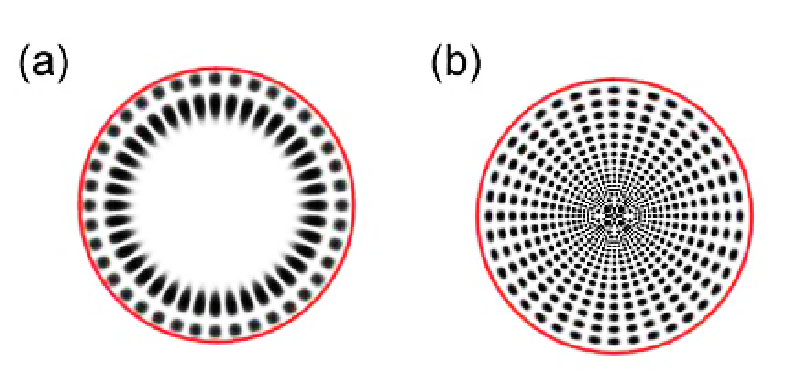
\includegraphics[width=5.5cm]{neg_ref_45}
\end{center}

Состояния с высокими угловыми моментами для изотропной среды (а) и среды с $\epsilon_r<0$, а
$\epsilon_{\theta}>0$. Поле проникает в сердцевину!

\end{columns}

\begin{center}
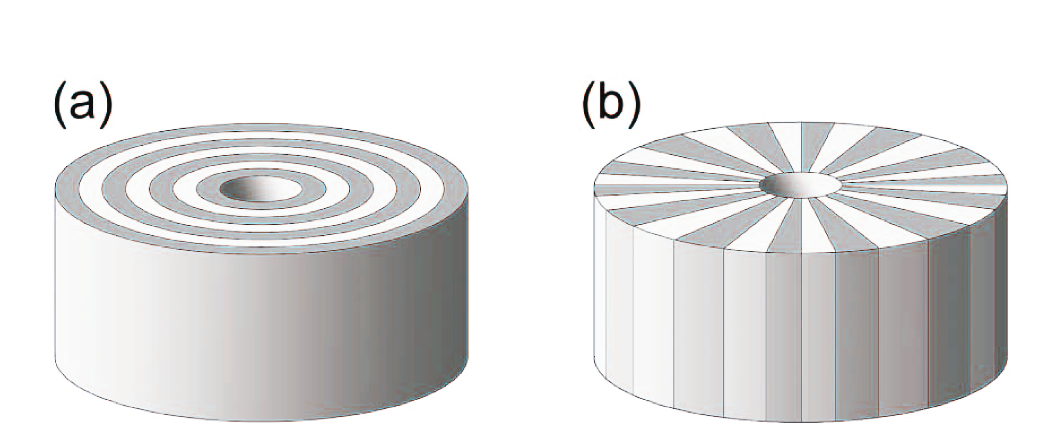
\includegraphics[width=5.5cm]{neg_ref_46}
\end{center}

 Возможные реализации метацилиндров.

\end{frame}

\begin{frame}{Сравнение результатов гиперлинзы и обычного материала}
\begin{center}
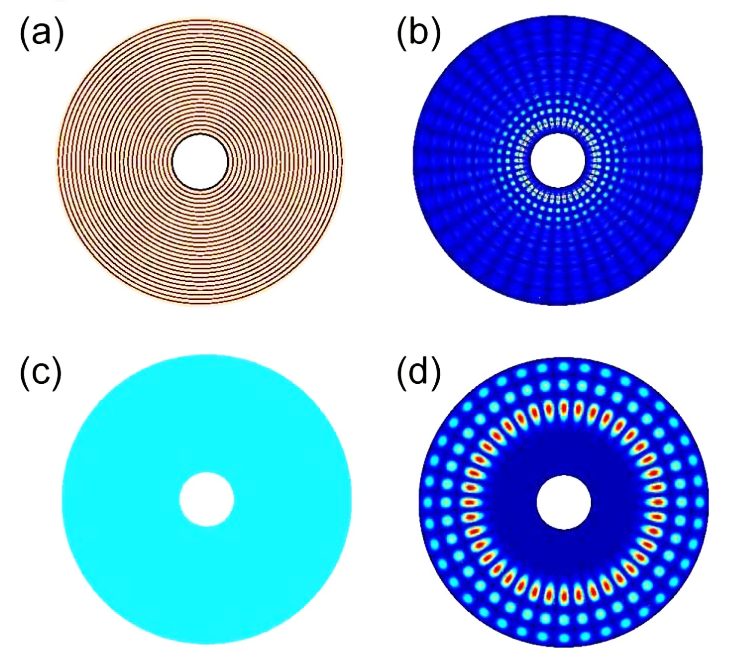
\includegraphics[width=5.5cm]{neg_ref_47}
\end{center}

Модель 50 слоев металла и диэлектрика $\epsilon_m = -2$ и диэлектрика $\epsilon_m = 5$.
Внешний радиус $2.2 \mu$м, внутренний $250$ нм. Расчет для $m=20$. То же но для изотропного
вещества $\epsilon_{uni} = 1.5$.

 Два точечных разделены расстоянием $\lambda/3$, 160 слоев, металл: $\epsilon_m
=-1+0.01 \imath $, диэлектрик $\epsilon_d = 1.1$, $R_{inner} =250$ нм, $R_{outer} = 1840$ нм

\end{frame}

\begin{frame}{Диполь в АММ}
\begin{center}
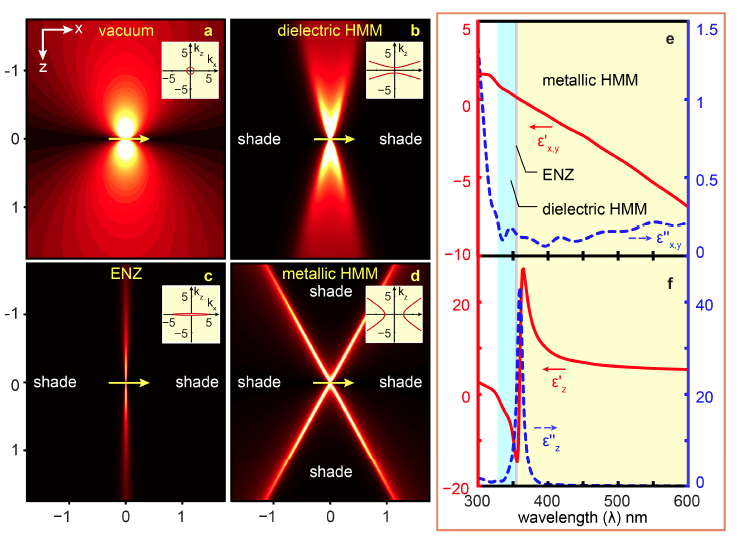
\includegraphics[width=\textwidth]{neg_ref_n13}
\end{center}
\end{frame}

\begin{frame}{Классификация плазмонных материалов}
\begin{center}
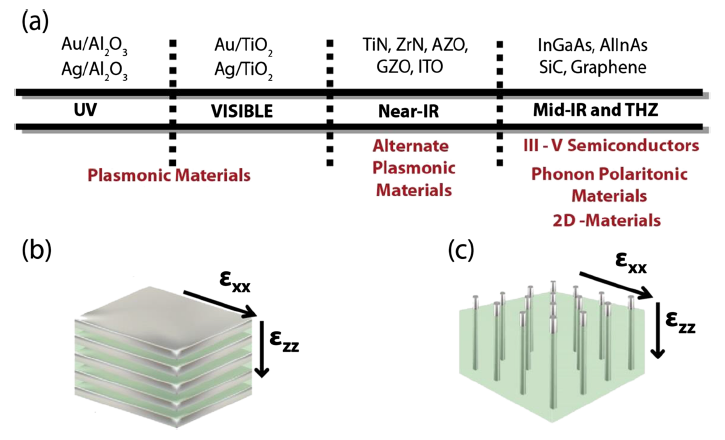
\includegraphics[width=\textwidth]{neg_ref_n6}
\end{center}
\end{frame}

\begin{frame}{Природные гиперболические метаматериалы}
графит, кальцит ($CaCo_3$), висмут
\begin{columns}[c]
\column{2.0in}
\begin{center}
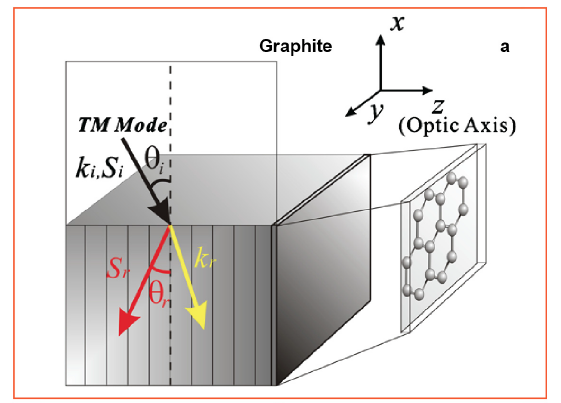
\includegraphics[width=\textwidth]{neg_ref_n14}
\end{center}
\column{2.0in}
\begin{center}
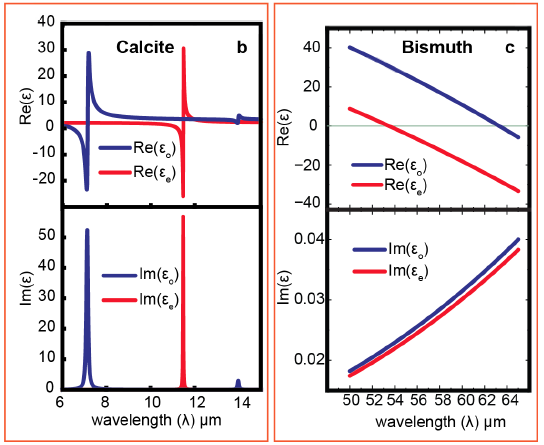
\includegraphics[width=\textwidth]{neg_ref_n16}
\end{center}
\end{columns}
У графита

 У кальцита

\end{frame}

\begin{frame}{Предварительные итоги}

\begin{center}
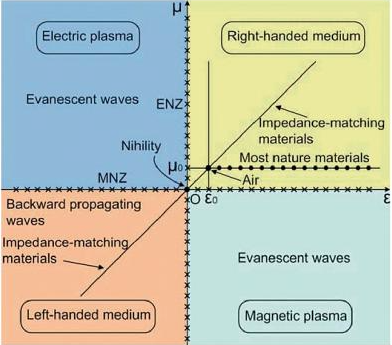
\includegraphics[width=0.5\textwidth]{neg_ref_n11}
\end{center}
В настоящее время от пассивных метаматериалов переходят к исследованию активных метаматериалов, т.е. таких, принцип работы которых во многом аналогичен работе лазера (т.н. спазеры).
\end{frame}

\end{document}


\begin{frame}{}


\begin{columns}[c]
\column{2.0in}
\begin{center}
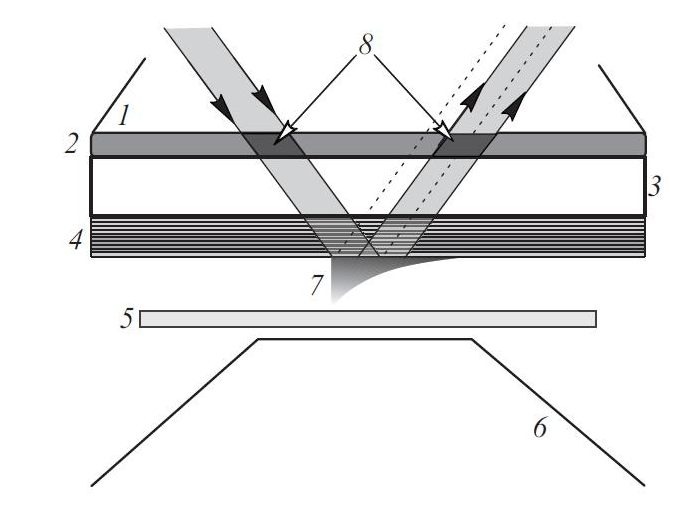
\includegraphics[scale=0.3]{gh4a}
\end{center}
\column{2.0in}
\begin{center}
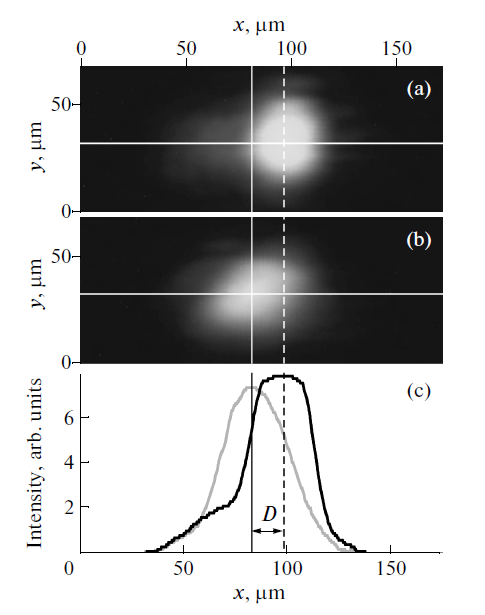
\includegraphics[scale=0.35]{gh4}
\end{center}


\end{columns}

\end{frame}





